\documentclass[a4paper]{article}
\newcommand{\sepspace}{\vspace*{1em}}	
%% Language and font encodings
\usepackage[english]{babel}
\usepackage[utf8x]{inputenc}
\usepackage[T1]{fontenc}
\usepackage{float}

%% Sets page size and margins
\usepackage[a4paper,top=3cm,bottom=2cm,left=3cm,right=3cm,marginparwidth=1.75cm]{geometry}

\usepackage{amsmath}
\usepackage{graphicx}

\title{ZND detonation of hydrogen and air}
\author{Mateusz Klos}

\begin{document}
\maketitle


\section{Introduction}\label{sec:intro}
In this report one will find a study about ZND detonation using mixture of air and hydrogen. There is a connection between detonation cell size and induction time, which will be calculated in this paper. This program calculates induction for equivalence ratio varying from 0.7 to 2.03. Calculation are performed using SDToolbox on Matlab.
\section{Mathematical model}\label{sec:model}
The ZND detonation model is a one-dimensional model for the process of detonation of an explosive. It was proposed during World War II independently by Y. B. Zel'dovich, John von Neumann, and Werner Döring, hence the name.

This model admits finite-rate chemical reactions and thus the process of detonation consists of the following stages. First, an infinitely thin shock wave compresses the explosive to a high pressure called the von Neumann spike. At the von Neumann spike point the explosive still remains unreacted. The spike marks the onset of the zone of exothermic chemical reaction, which finishes at the Chapman-Jouguet state. After that, the detonation products expand backward.
\section{Results}\label{sec:results}

\begin{figure}[H]
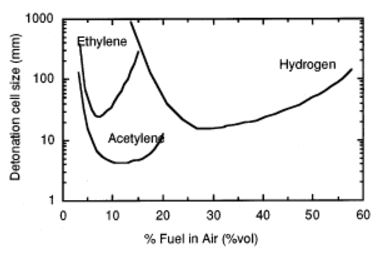
\includegraphics[width=1\textwidth]{hydrogen_figure.JPG}
\caption{\label{fig:cj}Experimental data}
\end{figure}

\begin{figure}[H]
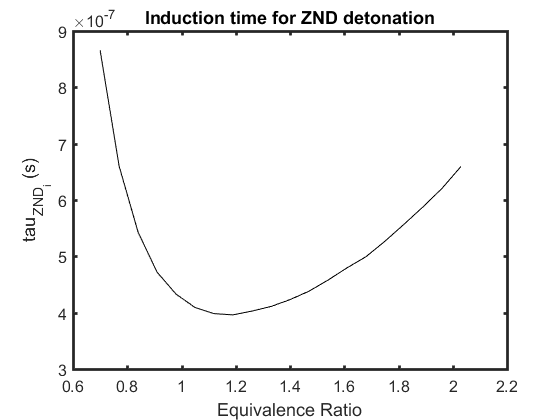
\includegraphics[width=1\textwidth]{znd_it.png}
\caption{\label{fig:p}Calculated ZND detonation}
\end{figure}

These two charts has similar properties, there is a relation which will be calculated below:

\begin{equation}
    a = t_ind/\lambda=3.98*10^{-7}/0,0117=3.4*10^{-5}
 \end{equation}   

\section{Summary}\label{sec:summary}
 Induction time was measured in $seconds^{-7}$. Results acquired from Matlab are close to experimental data.



\end{document}
